% 45 minutes, should be ~30 slides or so
\section{Basic Tutorials}

\begin{frame}{Virtual Machine Check}
How are we doing with the Virtual Box images?
\end{frame}

\begin{frame}{Ubuntu Introduction}
\begin{itemize}
  \item User experience oriented version of Linux
  \item Familiar desktop paradigm
  \item TODO: finish after image is ready
\end{itemize}
\end{frame}

\begin{frame}{Ubuntu - Hands On  }
\begin{itemize}
  \item TODO: what do we need to talk about here?
\end{itemize}
\end{frame}

\begin{frame}{Just Enough Python to be Dangerous}
\begin{itemize}
  \item Start a terminal
  \item Run iPython
\end{itemize}
\begin{center}
  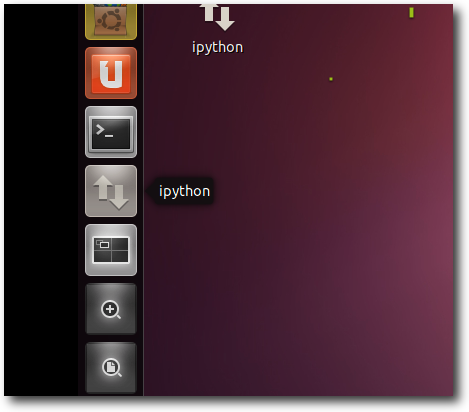
\includegraphics[width=0.5\textwidth]{Images/iPythonLaunch_shadow}
\end{center}
\end{frame}

\begin{frame}{Just Enough Python to be Dangerous}
\begin{center}
  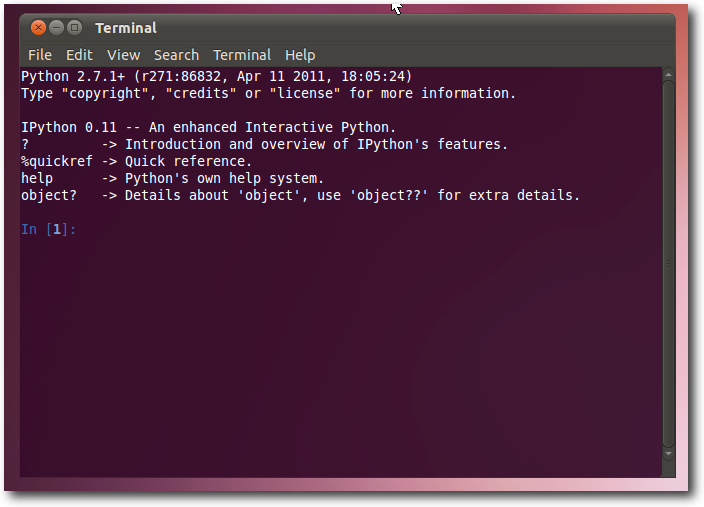
\includegraphics[width=0.5\textwidth]{Images/iPythonWindow_shadow}
\end{center}
\end{frame}

\begin{frame}{Just Enough Python to be Dangerous}
Import the SimpleITK package
\begin{center}
  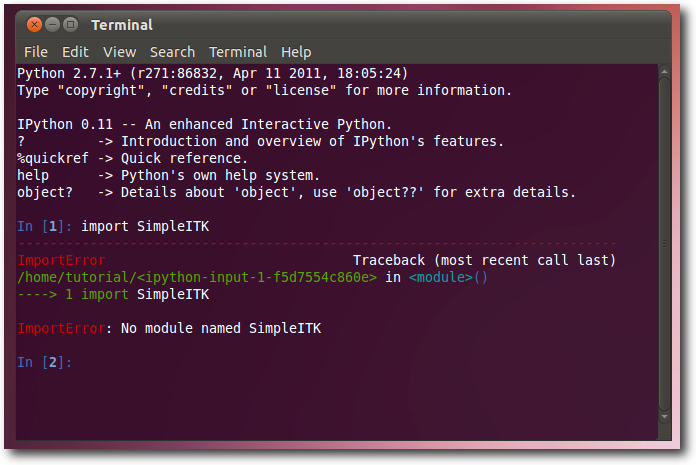
\includegraphics[width=0.5\textwidth]{Images/iPythonImportError_shadow}
\end{center}
What just happened?
\end{frame}

\begin{frame}{Just Enough Python to be Dangerous}
Need to tell iPython where to find SimpleITK\\
See /home/tutorial/.ipython/ipython.py
\begin{center}
  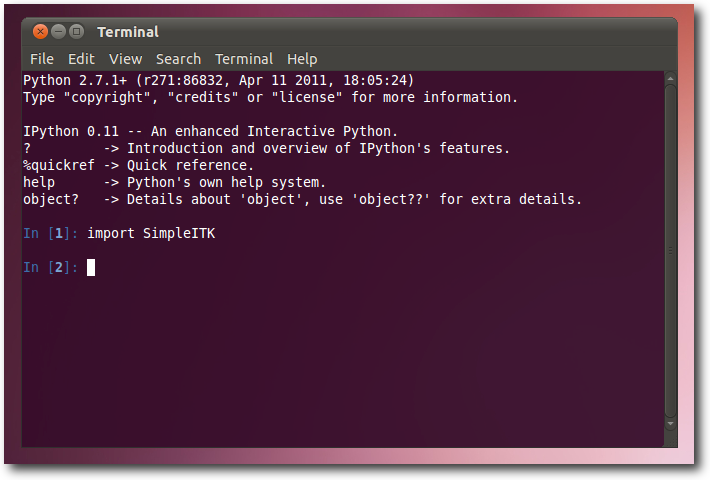
\includegraphics[width=0.5\textwidth]{Images/iPythonWithSimpleITK_shadow}
\end{center}
\end{frame}

\subsection{Image Basics}

\begin{frame}
\frametitle{Image Class}
\begin{itemize}
  \item Creation
  \item Number of dimensions, size, origin, spacing
  \item Pixel access
\end{itemize}
\end{frame}

% Must use the [fragile] option!
\begin{frame}[fragile]
\frametitle{What just happened?}
\lstpython
\begin{lstlisting}
# Create an image
image = SimpleITK.Image ( 256, 256, 256,
                          SimpleITK.sitkInt16 );
\end{lstlisting}

\begin{itemize}
  \item SimpleITK is the module
  \item Image is the constructor for the Image class
  \item Height, width, depth (omit depth for 2D images)
  \item Datatype (more on this later)
\end{itemize}

\end{frame}


\begin{frame}[fragile]
\frametitle{What just happened?}
\lstpython
\begin{lstlisting}
# Addressing pixels
image.GetPixel ( 0, 0, 0 )
image.SetPixel ( 0, 0, 0, 1 )
image.GetPixel ( 0, 0, 0 )
\end{lstlisting}
\begin{itemize}
  \item Get the voxel value at [0,0,0]?
  \item Hmm, I don't like it, so set to 1
  \item What is the value at [0,0,0] now?
\end{itemize}
\end{frame}

\begin{frame}[fragile]
\frametitle{What just happened?}
\lstpython
\begin{lstlisting}
# Addressing pixels
image[0,0,0]
image[0,0,0] = 10
image[0,0,0]
\end{lstlisting}
Without warning, we sprinkled syntatic sugar on you!
\begin{itemize}
  \item image[0,0,0] is shorthand for Image.GetPixel(0,0,0)
  \item image[0,0,0] = 10 is shorthand for Image.SetPixel(0,0,0,1)
\end{itemize}
\end{frame}

\begin{frame}[fragile]
\frametitle{Summary}
\begin{itemize}
  \item Images are created using SimpleITK.Image ( w, h, d, Type )
  \item Images can be 2- or 3-dimensional
  \item Images can describe themselves
  \item Images have simple pixel accessors
\end{itemize}
Questions before we move on?
\end{frame}

\subsection{Code Philosophy}
\begin{frame}{Code Philosophy}
\fontsize{36pt}{36pt}\selectfont
\center
\begin{center}
Code Philosophy
\end{center}
\end{frame}

\begin{frame}[fragile]
\frametitle{Object Paradigm (C++)}
\lstcpp
\begin{lstlisting}
#include <SimpleITK.h>
using itk::simple;
...
// Create a smoothing filter
SmoothingRecursiveGaussianImageFilter gaussian;
// Set a parameter
gaussian.SetSigma ( 2.0 );
// "Execute" the Filter
Image blurredImage = gaussian.Execute ( image );
\end{lstlisting}
\end{frame}

\begin{frame}[fragile]
\frametitle{Object Paradigm (C++)}
Flexibility
\lstcpp
\begin{lstlisting}
#include <SimpleITK.h>
using itk::simple;
...
// Create a smoothing filter
SmoothingRecursiveGaussianImageFilter gaussian;
// Set a parameter, then execute
Image blurredImage = gaussian
                       .SetSigma ( 2.0 )
                       .Execute ( image );
\end{lstlisting}
\end{frame}

\begin{frame}[fragile]
\frametitle{Object Paradigm (C++)}
\lstcpp
\begin{lstlisting}
#include <SimpleITK.h>
using itk::simple;
...
// Anonymous filter, parameters, execute
// Set a parameter, then execute
Image blurredImage = SmoothingRecursiveGaussianImageFilter()
                       .SetSigma ( 2.0 )
                       .SetRadius ( 5 )
                       .Execute ( image );
\end{lstlisting}
\end{frame}

\begin{frame}[fragile]
\frametitle{``Function'' Paradigm (C++)}
\lstcpp
\begin{lstlisting}
#include <SimpleITK.h>
using itk::simple;
...
// Call the function version
// NB: Drop the "ImageFilter"!
// Signature:
/*
    Image SmoothingRecursiveGaussian ( const Image&,
      double inSigma = 1.0,
      bool inNormalizeAcrossScale = false );
*/
Image blurredImage = SmoothingRecursiveGaussian (
                        image,
                        2.0,
                        false );
\end{lstlisting}
\end{frame}

\begin{frame}[fragile]
\frametitle{Mix \& Match (C++)}
\lstcpp
\begin{lstlisting}
#include <SimpleITK.h>
using itk::simple;
...
// Get our gaussian ready
SmoothingRecursiveGaussianImageFilter gaussian;
gaussian.SetSigma ( 2.0 );

// What is the effect on the image
Image difference = Subtract (
                     image,
                     gaussian.Execute ( image )
                     );
Image difference2 = Subtract (
                     image,
                     SmoothingRecursiveGaussian (
                       image, 2.0
                       )
                     );

\end{lstlisting}
\end{frame}


\begin{frame}{Other Languages}
\fontsize{36pt}{36pt}\selectfont
\center
\begin{center}
Other Languages
\end{center}
\end{frame}

\begin{frame}[fragile]
\frametitle{Object Paradigm (Python)}
The paradigms translate to the wrapped languages (C++ $\rightarrow$ Python)
\lstcpp
\begin{lstlisting}
#include <SimpleITK.h>
using itk::simple;
...
// Create a smoothing filter
SmoothingRecursiveGaussianImageFilter gaussian;
// Set a parameter
gaussian.SetSigma ( 2.0 );
// "Execute" the Filter
Image blurredImage = gaussian.Execute ( image );
\end{lstlisting}
\lstpython
\begin{lstlisting}
from SimpleITK import *
# Create a smoothing filter
SmoothingRecursiveGaussianImageFilter gaussian
# Set a parameter
gaussian.SetSigma ( 2.0 );
# "Execute" the Filter
blurredImage = gaussian.Execute ( image );
\end{lstlisting}
\end{frame}

\begin{frame}[fragile]
\frametitle{Object Paradigm (Java)}
\lstjava
\begin{lstlisting}
import SimpleITK.*;
...
// Create a smoothing filter
SmoothingRecursiveGaussianImageFilter gaussian =
      new SmoothingRecursiveGaussianImageFilter();
// Set a parameter
gaussian.SetSigma ( 2.0 );
// "Execute" the Filter
Image blurredImage = gaussian.Execute ( image );
\end{lstlisting}
\end{frame}


\begin{frame}{Note on the Tutorial}
\begin{itemize}
  \item Most examples will be Python
  \item Obvious translation to other languages
  \item C++ usage not (always) obvious
\end{itemize}
\end{frame}

%%%%%%%%%%%%%%
\subsection{Memory Management}

\begin{frame}{Memory Management}
\fontsize{36pt}{36pt}\selectfont
\center
\begin{center}
Memory Management
\end{center}
\end{frame}


\begin{frame}{Images}
Images...
\begin{itemize}
  \item usually allocated on the stack
  \item are copy-on-write
  \item use internal smart-pointers
\end{itemize}
\end{frame}

\begin{frame}[fragile]
\frametitle{Image Memory Management}
\lstpython
\begin{lstlisting}
image = SimpleITK.Image ( 32, 32, 32, SimpleITK.sitkInt16 )
print image
...
Image (0x94f2d98)
  Reference Count: 1
...
# Clone image
b = SimpleITK.Image ( image )
print image
...
Image (0x94f2d98)
  Reference Count: 2
...
print b
...
Image (0x94f2d98)
\end{lstlisting}
\end{frame}

\begin{frame}[fragile]
\frametitle{Image Memory Management}
\lstpython
\begin{lstlisting}
print b
...
Image (0x94f2d98)
...
b[0,0,0] = 1
print b
...
Image (0x94f4cb0)
  Reference Count: 1
...
print image
...
Image (0x94f2d98)
  Reference Count: 1
...
\end{lstlisting}
\end{frame}


\begin{frame}{Filters}
Filters...
\begin{itemize}
  \item usually allocated on the stack
  \item tend to clean up after themselves
  \item do not hold on to images
\end{itemize}
\end{frame}

\begin{frame}{Memory Management Strategies}
C++\dots
\begin{itemize}
  \item No need for explicit management
  \item Let images clean up after themselves
  \item Let filters clean up after themselves
\end{itemize}
Wrapped\dots
\begin{itemize}
  \item Utilize language-specific memory management
  \item Automatic in Python, Java, Ruby, C\#, Lua
  \item More manual in Tcl
\end{itemize}
\end{frame}

%%%%%%%%%%%%%%
\subsection{Input/Output}

\begin{frame}{Input/Output}
\fontsize{36pt}{36pt}\selectfont
\center
\begin{center}
Input/Output
\end{center}
\end{frame}

\begin{frame}{Read/Write/Display Images}
  Back to iPython
\end{frame}

\begin{frame}[fragile]
\frametitle{Display}
\begin{center}
  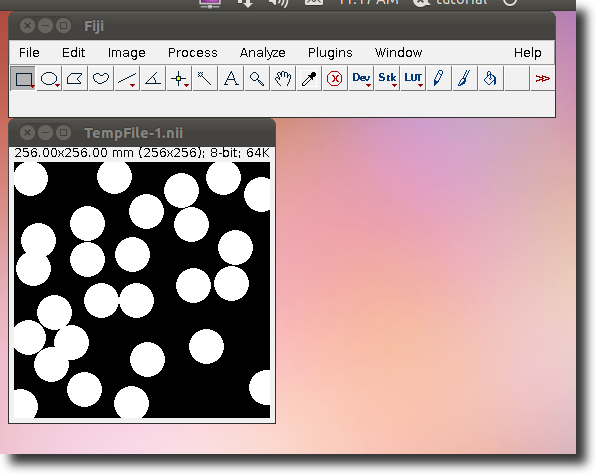
\includegraphics[width=0.5\textwidth]{Images/ImageDisplay_shadow}
\end{center}

What just happened?
\lstpython
\begin{lstlisting}
# What's the image look like?
SimpleITK.Show ( image )
\end{lstlisting}
\end{frame}

\begin{frame}[fragile]
\frametitle{Display}
\begin{columns}[c]
\column{0.4\textwidth}
\begin{center}
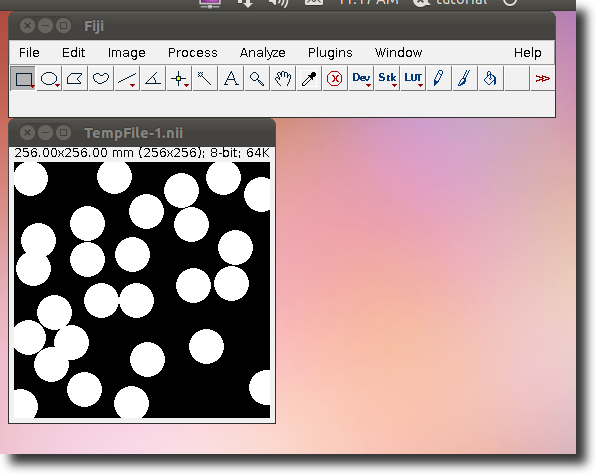
\includegraphics[width=1\textwidth]{Images/ImageDisplay_shadow} \\
Ubuntu
\end{center}
\column{0.4\textwidth}
\begin{center}
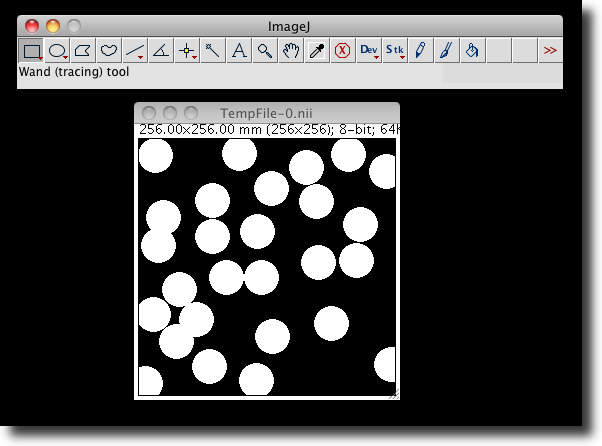
\includegraphics[width=1\textwidth]{Images/ImageDisplayMac_shadow} \\
Mac
\end{center}
\end{columns}
\begin{itemize}
  \item ImageJ/Fiji used for display
  \item SimpleITK looks in most likely location for ImageJ
  \item Image written in Nifti format
  \item Need to install Nifti plugin for ImageJ
  \item \url{http://rsbweb.nih.gov/ij/plugins/nifti.html}
\end{itemize}
\end{frame}




